\documentclass[11pt]{article}
\usepackage[utf8]{inputenc}
\usepackage[T1]{fontenc}
\usepackage{amsmath}
\usepackage{amssymb}
\usepackage{multicol}
\usepackage{geometry}
\usepackage{tikz}
\usepackage{enumitem}
\usepackage{xcolor}
\usepackage{titlesec}
\usetikzlibrary{shadows}
\usepackage{graphicx}
\usepackage{ragged2e}

% Configurações de layout
\geometry{a4paper, left=1cm, right=1cm, top=0.5cm, bottom=1.2cm}
\setlength{\columnseprule}{0.4pt}

% Cores para títulos
\titleformat{\section}{\normalfont\Large\bfseries\color{blue}}{\thesection}{1em}{}
\titleformat{\subsection}{\normalfont\large\bfseries\color{red}}{\thesubsection}{1em}{}

\title{\textcolor{blue}{Cultura Digital \\ Cibersegurança e Ética Digital em ``Mr. Robot''}}
\author{Professor: Jefferson}
\date{}

\begin{document}

\maketitle
\vspace{-1cm}

\begin{center}
\large{Nome: \underline{\hspace{8cm}} \quad Turma: \underline{\hspace{3cm}}}
\end{center}

\begin{multicols}{2}

\section*{Objetivo da Aula}

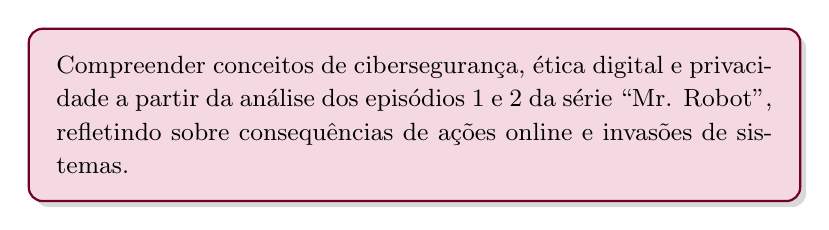
\begin{tikzpicture}
\node[rectangle, 
      fill=purple!15, 
      rounded corners=5pt, 
      inner sep=10pt, 
      draw=purple!60!black, 
      thick,
      drop shadow={opacity=0.3},
      text width=0.75\linewidth,
      align=justify] 
{
\small
 Compreender conceitos de cibersegurança, ética digital e privacidade a partir da análise dos episódios 1 e 2 da série ``Mr. Robot'', refletindo sobre consequências de ações online e invasões de sistemas.
};
\end{tikzpicture}

\vspace{5mm}

\section*{1. Introdução}

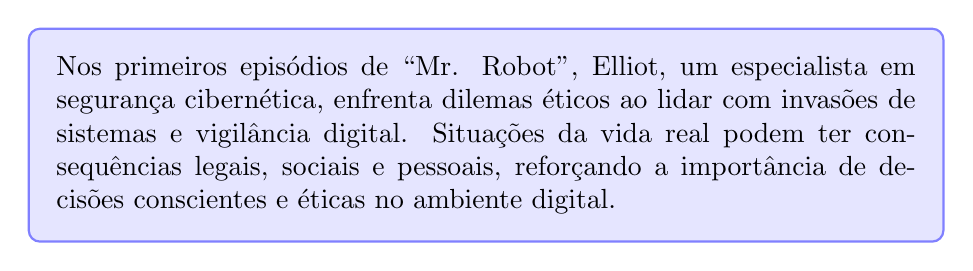
\begin{tikzpicture}
\node[rectangle, fill=blue!10, rounded corners, inner sep=10pt, draw=blue!50, thick, text width=0.9\linewidth, align=justify] {
Nos primeiros episódios de ``Mr. Robot'', Elliot, um especialista em segurança cibernética, enfrenta dilemas éticos ao lidar com invasões de sistemas e vigilância digital. Situações da vida real podem ter consequências legais, sociais e pessoais, reforçando a importância de decisões conscientes e éticas no ambiente digital.
};
\end{tikzpicture}

\vspace{5mm}

\section*{2. Conceitos Fundamentais}

\subsection*{Segurança de Dados}

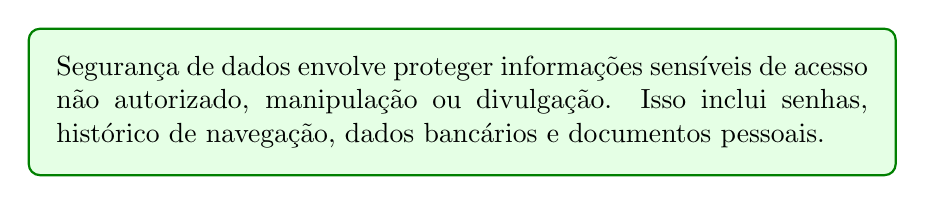
\begin{tikzpicture}
\node[rectangle, fill=green!10, rounded corners, inner sep=10pt, draw=green!50!black, thick, text width=0.85\linewidth, align=justify] {
Segurança de dados envolve proteger informações sensíveis de acesso não autorizado, manipulação ou divulgação. Isso inclui senhas, histórico de navegação, dados bancários e documentos pessoais.
};
\end{tikzpicture}

\vspace{3mm}

\subsection*{Ética Digital}

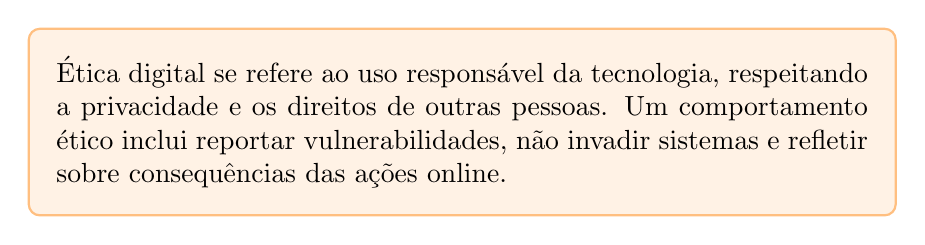
\begin{tikzpicture}
\node[rectangle, fill=orange!10, rounded corners, inner sep=10pt, draw=orange!50, thick, text width=0.85\linewidth, align=justify] {
Ética digital se refere ao uso responsável da tecnologia, respeitando a privacidade e os direitos de outras pessoas. Um comportamento ético inclui reportar vulnerabilidades, não invadir sistemas e refletir sobre consequências das ações online.
};
\end{tikzpicture}

\vspace{5mm}

\section*{3. Atividade Prática}

\textbf{Cenário:} Inspirado em ``Mr. Robot'', você encontrou uma falha em um sistema corporativo que poderia expor dados sensíveis de milhares de pessoas.

\begin{enumerate}[leftmargin=*]
\item Liste duas ações que você poderia tomar diante dessa situação e explique por que são éticas ou antiéticas.\\[4\baselineskip]

\item Quais medidas de proteção digital você aplicaria para proteger suas próprias informações e as de terceiros?\\[4\baselineskip]

\item Imagine que você acessou um fórum de hackers e encontrou dados de outras pessoas. Como você deveria agir de acordo com a ética digital?\\[4\baselineskip]
\end{enumerate}

\vspace{5mm}

\section*{4. Dicas de Segurança}

\begin{center}
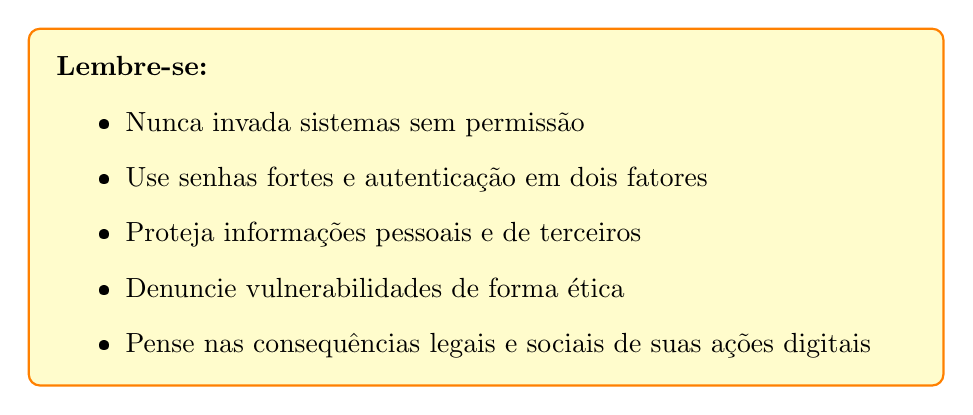
\begin{tikzpicture}
\node[rectangle, fill=yellow!20, rounded corners, inner sep=10pt, draw=orange, thick, text width=0.9\linewidth, align=justify] {
\textbf{Lembre-se:}
\begin{itemize}
\item Nunca invada sistemas sem permissão
\item Use senhas fortes e autenticação em dois fatores
\item Proteja informações pessoais e de terceiros
\item Denuncie vulnerabilidades de forma ética
\item Pense nas consequências legais e sociais de suas ações digitais
\end{itemize}
};
\end{tikzpicture}
\end{center}

\section*{5. Questões}

\begin{enumerate}[leftmargin=*]

\item Qual atitude representa um comportamento ético no ambiente digital?
\begin{enumerate}[label=\alph*)]
\item Invadir sistemas para ganhar informações pessoais.
\item Reportar falhas de segurança para responsáveis.
\item Divulgar dados de terceiros em redes sociais.
\item Compartilhar senhas de outras pessoas.
\end{enumerate}

\item O que significa segurança de dados?
\begin{enumerate}[label=\alph*)]
\item Proteção de informações sensíveis contra acessos não autorizados.
\item Publicação de dados em redes sociais.
\item Uso de senhas simples para todos os sites.
\item Instalar apenas antivírus gratuito.
\end{enumerate}

\item Qual é a principal preocupação ética de um hacker ético?
\begin{enumerate}[label=\alph*)]
\item Roubar informações confidenciais.
\item Expor falhas publicamente para prejudicar alguém.
\item Proteger sistemas e agir dentro da lei.
\item Aumentar seguidores online.
\end{enumerate}

\item Por que é importante refletir antes de postar informações online?
\begin{enumerate}[label=\alph*)]
\item Para evitar ataques cibernéticos e proteger a privacidade.
\item Para ganhar mais curtidas.
\item Para aumentar seguidores.
\item Para reduzir uso de senhas.
\end{enumerate}

\item Qual medida ajuda a proteger dados pessoais?
\begin{enumerate}[label=\alph*)]
\item Criar senhas fortes e únicas.
\item Compartilhar senhas com amigos.
\item Postar dados sensíveis em fóruns.
\item Ignorar atualizações de segurança.
\end{enumerate}

\item Nos episódios iniciais de ``Mr. Robot'', Elliot decide invadir sistemas para descobrir fraudes. Qual é o principal risco dessa ação?
\begin{enumerate}[label=\alph*)]
\item Melhorar sua reputação online.
\item Consequências legais, exposição de dados e risco à ética pessoal.
\item Aumentar seguidores em redes sociais.
\item Receber elogios de empresas.
\end{enumerate}

\item O que é phishing, prática vista na série como tentativa de enganar usuários?
\begin{enumerate}[label=\alph*)]
\item Um tipo de ataque que coleta informações pessoais através de engano.
\item Um programa de proteção de dados.
\item Um tipo de senha segura.
\item Um software de criptografia avançada.
\end{enumerate}

\item Qual prática de segurança Elliot poderia usar para proteger suas contas e dados pessoais?
\begin{enumerate}[label=\alph*)]
\item Senhas fracas para lembrar facilmente.
\item Autenticação em dois fatores e senhas fortes.
\item Compartilhar senhas apenas com amigos confiáveis.
\item Publicar todas as senhas em fóruns seguros.
\end{enumerate}

\item Quando se depara com informações sensíveis de terceiros, qual é a ação correta?
\begin{enumerate}[label=\alph*)]
\item Divulgar para alertar outras pessoas.
\item Ignorar a informação ou reportar de forma ética.
\item Vender as informações para obter lucro.
\item Usar as informações para influenciar decisões pessoais.
\end{enumerate}

\item Qual é a mensagem central sobre cibersegurança apresentada nos episódios 1 e 2 de ``Mr. Robot''?
\begin{enumerate}[label=\alph*)]
\item Tecnologia é sempre segura e confiável.
\item As decisões digitais têm impactos legais, éticos e sociais; segurança e ética devem caminhar juntas.
\item Hackers são sempre criminosos sem consequências.
\item Redes sociais não afetam a vida real.
\end{enumerate}


\end{enumerate}

\end{multicols}

\end{document}

